% 
% Annual Cognitive Science Conference
% Sample LaTeX Paper -- Proceedings Format
% 

%% Change "letterpaper" in the following line to "a4paper"e if you must.

\documentclass[10pt,letterpaper]{article}

\usepackage{cogsci}
% Recommended, but optional, packages for figures and better typesetting:
\usepackage[margin=1in]{geometry} 
\usepackage{microtype}
\usepackage{graphicx}
\usepackage{subfigure}
\usepackage{booktabs} % for professional tables
\usepackage{nicefrac}       % compact symbols for 1/2f, etc.
\usepackage{microtype}      % microtypography
\usepackage{float}
\usepackage[colorlinks,allcolors=purple]{hyperref}
\usepackage{algorithm}
\usepackage{amsmath}
\usepackage{graphicx}
\usepackage[table,xcdraw]{xcolor}
\usepackage{gensymb}
\usepackage{stmaryrd}
\usepackage{amssymb}
\usepackage{todonotes}
\usepackage{comment}

%\cogscifinalcopy % Uncomment this line for the final submission 
\newcommand{\jda}[1]{{\color{blue}[jda: #1]}}


\usepackage{pslatex}
\usepackage{apacite}


%\usepackage[none]{hyphenat} % Sometimes it can be useful to turn off
%hyphenation for purposes such as spell checking of the resulting
%PDF.  Uncomment this block to turn off hyphenation.


\setlength\titlebox{4.5cm}
% You can expand the titlebox if you need extra space
% to show all the authors. Please do not make the titlebox
% smaller than 4.5cm (the original size).
%%If you do, we reserve the right to require you to change it back in
%%the camera-ready version, which could interfere with the timely
%%appearance of your paper in the Proceedings.



% \title{Contextually-adapted abstractions explain \\ contextually-adapted abstraction in language} 
\title{Identifying concept libraries from language about object structure}
 
\author{{\large \bf Morton Ann Gernsbacher (MAG@Macc.Wisc.Edu)} \\
  Department of Psychology, 1202 W. Johnson Street \\
  Madison, WI 53706 USA
  \AND {\large \bf Sharon J.~Derry (SDJ@Macc.Wisc.Edu)} \\
  Department of Educational Psychology, 1025 W. Johnson Street \\
  Madison, WI 53706 USA}


\begin{document}

\maketitle


\begin{abstract} %% 148 words
Our understanding of the visual world goes beyond naming objects --- encompassing our ability to parse objects into meaningful parts, attributes, and relations. 
Here we leverage the language people use to describe a diverse collection of 2K novel objects to understand what parts they find meaningful, and reverse engineer why they favored these parts. 
We achieve this by formalizing our problem as search over the space of graphics libraries that contain different part concepts;
then evaluate how well programs written in each library explain human language.
While a library containing only the simplest shape primitives (e.g., block) explains some variance, we discover that libraries containing moderately complex part concepts (e.g., pillar) provide both efficient compression of these objects and better explain how people describe them.
Our findings highlight the value of measuring naturalistic language behavior at scale and using structured program representations for exposing how our perceptual 
experience is organized. 

%%% 183 words
% Our understanding of the visual world goes beyond naming objects --- encompassing the the organization of our perceptual experience into parts and relations. 
% Here we leverage the language people use to describe a diverse collection of 2K novel objects to understand what parts they find meaningful, and reverse engineer the principles that explain why they favored these part descriptors. 
% We achieve this by formalizing our problem as search over the space of graphics libraries that vary in the visual part concepts they contain. 
% We then evaluate how well the programs written in each library explain quantitative and qualitative patterns in human language.
% While we find that a ``base'' library containing only the simplest shape primitives (e.g., block) explains some variance in the length of linguistic descriptions, we discover that libraries containing moderately complex part concepts (e.g., pillar) provide both efficient compression of these objects and better explain the way people describe them.
% Taken together, our findings highlight the value of measuring naturalistic language behavior at scale and using structured program representations for exposing the perceptual units we use to make sense of the world. 
%%%

% Our understanding of the visual world goes beyond naming objects --- encompassing the parts and relations that constitute our internal representation of them.
% although any of these libraries could in principle be used to generate each object.
% To answer this question, we first designed a large and varied collection of 2K novel objects and elicited natural-language descriptions of them. 
% Next, we evaluated how well these descriptions could be explained by relating them to graphics programs written using only maximally simple shape primitives. 

% We found a systematic relationship between the number of words used to describe an object and the length of the program required to generate that object in a simple graphics library, as well systematic differences in the vocabularies used to describe objects in different categories.
% Next, we formalized our 

%%%%%
% In this paper, we introduce a large corpus of natural-language descriptions for multiple structured object domains ($4650$ descriptions across 2000 distinct objects) along with a novel translation-based approach for identifying concept libraries from language.
% First, we find a systematic relationship between the number of words required to describe an object and the length of the program required to generate that object in a domain-specific language (DSL), as well as a systematic difference in the vocabularies used to describe objects in different domains. 
% We then introduce a more expressive \textit{program-language alignment} approach, and find that language is best explained by concept libraries that jointly minimize program description length \textit{and} the underlying number of conceptual primitives in the DSL library.
% Taken together, our findings emphasize the intimate relationship between conceptual and linguistic representations and provides basis for further exposing the library of conceptual primitives we use to make sense of the world. 

% We experience the visual world as structured into objects and parts, and use language to communicate about that structure, even for entities we have never seen before.
% Our visual world is richly structured into meaningful objects and parts. 
% How do people extract and represent such structure?
% Naturalistic language production presents a promising window into these representations, as a medium adapted for communicating about structure, but it has been challenging to link candidate hypotheses about concept hierarchies to such data.
% In this paper, we introduce a large corpus of natural-language descriptions for multiple structured object domains ($4200$ descriptions across 2000 distinct objects) along with a novel translation-based approach for identifying concept libraries from language.
% First, we find a systematic relationship between the number of words required to describe an object and the length of the program required to generate that object in a domain-specific language (DSL), as well as a systematic difference in the vocabularies used to describe objects in different domains. 
% We then introduce a more expressive \textit{program-language alignment} approach, and find that language is best explained by concept libraries that jointly minimize program description length \textit{and} the underlying number of conceptual primitives in the DSL library.
% Taken together, our findings emphasize the intimate relationship between conceptual and linguistic representations and provides basis for further exposing the library of conceptual primitives we use to make sense of the world. 

% While we do flexibly shift our words to suit the needs of different contexts, the ways in which we do so when describing compositional phenomena is less well understood.
% In this paper we present a novel set of hierarchical stimuli, and present an experiment in which we elicited compositional descriptions of these stimuli in different contexts. 

\textbf{Keywords:} concepts; percepts; language; structure
\end{abstract}


%\section{Introduction} \label{sec-introduction}
% \textit{[CW: I will probably get to a major rewrite of this intro on *Saturday*. But earmarking that the main changes I'm *planning to make are*: to present the novel part of our work (with respect to the earlier work) as identifying the *vocabularies* people use across domains, rather than the individual words they use in free-naming tasks. that are characteristic of the basic level; in that way, what we have here is really a generalization of this notion of a default level of abstraction, extended to whole vocabularies used to discuss domains of complex scenes; and an information-theoretic hypothesis about DSL size + program length that we correlate with natural language vocabularies in Part II and Part III.]}

%% CW: jefan notes: rather than hypothesizing the basic level, i think it will be  more impactful to pose the theoretical question about representation-for-communication -- and reveal it through our library identification method, and discuss the basic-level thought as an implication at the end of the paper.
% RUNNING EXAMPLE: TBD? Needs to be some real world constructive task. 

% Examples of natural language communication of things with structure abound: | How to build a bike | How to build a house - windows, a door, |  ----We have specialized ways of talking about how to build a bike; your car; of a kitchen applicance; when we talk procedural tasks: furniture; people know about specialized words for recipes; ___; and for building architecture.\

%% 0: THE PHENOMENON: How do we talk about structure in the world? Give examples of talking about structure. 
%% 1: LITERATURE 1 Perceptual organization & visual concepts -- MEANINGS that carve up structure of the world.
%% the good: tradition of configural processing for many visual domains (objects; Biederman/Hummel; scenes: Melissa Vo)
%% the gap: a focus on holistic discrimination judgments rather than part structure -- % BUT: Most of this has been discrimination and labeling tasks. Not about structure; in complex scenes. -- and these have been point instance for instance-level language.
%% 2: LITERATURE 2 Constraints on communication -- LANGUEG / VOCABULARIES that carve the world.
%% the good: why do we have the vocabularies we do; and what are they bound to? the notion of negotiating a tradeoff between compression & expressivity %% \cite{kirby2015compression}, and many others.
%% the gap: those studies have been using artificial language (artificial tokens). small stimulus sets that don't vary that much in complexity and type. Really important limitations if we want to explain HOW people talk about structure. [Some of this is also less about structure (eg. color naming); others more about language evolution. But similar points about library size and compression.] -- and these have been point language for instance-level language.

%% 3: WHAT WE DID ABOUT IT: Formal link using program representations & library identification -- representational AND measurement innovations.)
    % WE propose a generic way of representing concepts (PROGRAMS)
%%  And: a linking function between program concepts to to REAL language. across broader variation in stimulus type & complexity. 
%%  what we learned and why LIT1 and LIT2 are both better off for it: perception people get structure; language people get where lexica come from (they carve at the joints of mental representations using this generic representational framework.) -- and this is a generic framework for doing this (exposing these information theoretic ideas)  AT SCALE for COMPLEX domains of stimuli. 
% Some nested clause mentioning: Ellis (?); Tian et. al; McCarthy et. al

% Our main contributions:
% LIT 1: A generic framework for discovering conceptual structure; our hypothesis space is over libraries. 
% LIT 2: Attempts to understand languages that emerge in iterated paradigms have been in restricted domains with low-stimulus variaiton and low-linguistic naturalism.
% People seem to communicate about structure. But how do we know what structure people actually represent? (Here, we have MUlTIPLE libraries that represent alternate hypotheses about structure -- what is the concept library people are actually using?) Prior work has evaluated SPECIFIC libraries.
% People seem to communicate this IN language. (This is a particularly good window into the mind of their thoughts about structure.) We ALSO have a library identification tool that tells you which ONES best fit their overt behavior in language.

The world is filled with a great variety of objects, yet people have little difficulty making sense of them. 
Presented with novel objects, people can readily identify their parts \cite{palmer1977hierarchical,marr1978representation, hoffman1984parts, hummel1992dynamic}, guess their functions \shortcite{tversky1984objects}, and refer to them unambiguously \cite{hawkins2020characterizing}. 
These abilities rest on the ability to robustly connect features of the external world to a rich library of mental concepts describing not just objects, but their parts and relations \shortcite{miller2013language, landau1993and}. 

% how do we connect inputs to percepts
Predicting which parts people use to parse the visual world has been a core target for classic theories of perceptual organization \shortcite{palmer1977hierarchical,marr1978representation,hoffman1984parts,biederman1987recognition,hummel1992dynamic} and continues to pose challenges for modern vision models \shortcite{mo2019partnet, bear2020learning, hinton2021represent}.
However, empirical tests of these proposals have generally relied upon simple discrimination tasks rather than richer behavioral readouts, limiting their ability to evaluate detailed correspondences between each putative representation and the full set of parts and relations that people can identify.
Further progress on these questions may thus benefit from embracing the use of more naturalistic and complex readout tasks for achieving higher resolution into the content and structure of perceptual representations \shortcite{sun2021seeing, mukherjee2019communicating}. 


% \jda{someone fill in: what is a concept, and what does it mean to ``have'' a concept}
Consider the bottom-most \emph{gadget} in Fig.~\ref{fig:task}A: even though this object does not correspond to a familiar category, it is easy to guess that it contains a row of \texttt{buttons} or \texttt{dials}, and that it is topped by an \texttt{antenna} or a \texttt{knob}.
But just as we do not have a pre-existing concept for every object we encounter, we do not have a concept corresponding to every part or feature: in Fig.~\ref{fig:task}A, for example, most people do not have a concept corresponding to a \texttt{row of exactly five dials}, or a \texttt{box with an antenna on top}. 

Indeed, a complex object can in principle be decomposed in many different ways, but that does not mean that people . What characterizes the set of concepts that humans \emph{do} have? Why these, and not others?
% Indeed, a complex object can be decomposed into combinatorially many substructures like these, but a typical human will analyze an object using only a tiny subset of these. What characterizes the set of concepts that humans \emph{do} have? Why these, and not others?




% how do we connect from percepts to linguistically expressible concepts?
% Meanwhile, it is not obvious which level of abstraction  relevant for characterizing its structure.






% How do people actually decompose these objects when describing their structure? And what are the principles that explain why they decompose them one way instead of another?
% There is considerable evidence that languages have been shaped by communicative need to expose relevant structure in the world \shortcite{rosch1976basic, tversky1984objects}. 
% We do not have words for every possible part decomposition, hence the parts that do become lexicalized in our vocabulary may be the product of resolving a tradeoff between informativeness and cognitive economy \shortcite{regier201511,kirby2015compression,zaslavsky2018efficient}.



This paper seeks to answer both questions. 
To do so, we use \emph{language} as a source of evidence for the human concept library, and \emph{programs} as representations of the internal structure of concepts. Both components of this approach have a long history in cognitive science: 

%%%%%%
% \jda{someone fill this in: not exactly the regier et al cites, but instead support for the claim ``has a lexicon entry'' = ``has a concept''}. 
% \jda{what's new about our synthesis of these tools? relative to the efficient comm literature, something like ``we're not just studying words, but the internal structure of the concepts they specify''}
%%%%%%

In \textbf{Part I}, we describe a procedure for generating complex but naturalistic visual stimuli that can be described by programs. Using this procedure, we collect a large dataset of images paired with both programmatic and natural language descriptions. Analyzing these descriptions reveals a distinctive feature of the concept library: individual concepts are \emph{boundedly complex}, and as stimuli grow more complex, their descriptions become \emph{longer} rather than reliant on more complex concepts.
In \textbf{Part II}, we refine this picture of the concept library. We show that a preference for bounded concept complexity is not arbitrary, but instead reflects a fundamental trade-off between the complexity of the library and the complexity of individual object analyses. We show that human lexical choice is best explained by libraries that \emph{optimize a description length criterion}: minimizing the length of all the programs in the library plus the length of an average stimulus expressed in terms of those programs.

%%%%%%
% \jda{This is also a place we could distinguish what we're doing from noga/terry r/ted g-type work}
%%%%%%

Together, these results suggest that the human concept inventory, like \jda{someone fill in: various other aspects of human cognition}, reflects a sophisticated trade-off between complexity and explanatory adequacy, and that the internal structure of concepts (modeled as programs and revealed in lexical choice) is an important component of this trade-off.

\begin{comment}

%%%% PHENOMENON: How do we talk about structure in the world? 
\noindent The world is filled with a great variety of objects, yet people have no trouble finding ways to talk about them. 
People not only know what to call a given object, but also how to describe its structure --- what parts it is composed from and how those parts are arranged.
% In other words, the underlying structure of our percepts and concepts is often reflected in the structure of our language \cite{miller2013language,landau1993and}.
In other words, our experience of structure in the visual world and the language we use to communicate about it appear to be closely coupled \cite{miller2013language,landau1993and}.
For example, a car has a \emph{body}, \emph{windows}, \emph{doors}, and \emph{wheels}.
Houses also have \emph{doors} and \emph{windows} (even if they look different from those of cars), but may be multiple \emph{stories} and have a \emph{roof} on top.
Even for an object someone has never seen before, people can generally figure out how to describe it so that they are understood \cite{hawkins2020characterizing}. 
What does the way we talk about objects reveal about how their structure is represented in the mind?

% What  enable people to so robustly communicate their understanding of how objects are organized?

%%%% PERCEPTION
Uncovering the perceptual units by which people parse the visual world has been a core target for classic theories of perception \shortcite{palmer1977hierarchical,marr1978representation,hoffman1984parts,hummel1992dynamic} and continues to pose challenges for modern vision models \shortcite{mo2019partnet, bear2020learning, hinton2021represent}.
Proposed solutions have varied widely, from defining a fixed set of volumetric primitives \shortcite{biederman1987recognition}, to using dimensionality reduction \shortcite{lee1999learning} or probabilistic inference \shortcite{austerweil2013nonparametric} to recover a part basis over image-like representations.
However, empirical tests of these proposals have largely been limited to simple discrimination or judgment tasks, limiting their ability to evaluate detailed correspondences between each putative representation and the full set of parts and relations that people can identify.
% making it challenging to evaluate the precise abstractions being used at an instance-by-instance level. 

%%%% LANGUAGE
Natural language behavior may provide a promising alternative way to access these representations. 
For example, consider the drawings in the left column of Fig. \ref{fig:task}A.
Someone could fully describe each drawing in terms of a few basic shapes (e.g., \textit{lines, circles}), by using names for larger units (e.g., \textit{dial}, \textit{drawer}), or even by producing a single phrase that refers to multiple parts.
How do people actually decompose these objects when describing their structure? And what are the principles that explain why they decompose them one way instead of another?
There is considerable evidence that languages have been shaped by communicative need to expose relevant structure in the world \shortcite{rosch1976basic, tversky1984objects}. 
We do not have words for every possible part decomposition, hence the parts that do become lexicalized in our vocabulary may be the product of resolving a tradeoff between informativeness and cognitive economy \shortcite{regier201511,kirby2015compression,zaslavsky2018efficient}.
% Meanwhile, many other visual motifs are more costly to express in words.

To explore this possibility, here we leverage the language people use to describe a large and varied set of novel objects to uncover the part concepts that people deem most relevant for characterizing their structure.
We formalize our problem as search over the space of graphics libraries that vary in the visual part concepts they contain, building on recent work in program library discovery \shortcite{ellis2020dreamcoder,tian2020learning, wang2021learning}.
We then evaluate how well the programs written in each library predict how much and what people say (Fig.~\ref{fig:task}B).
% explain quantitative and qualitative patterns in human language.
While a ``base'' library containing only the simplest shape primitives (e.g., block) explains some variance in the length of linguistic descriptions, we found that libraries containing moderately complex part concepts (e.g., pillar) provide both efficient compression of these objects and better explain the way people describe them.

\end{comment}
% Taken together, our findings highlight the value of measuring naturalistic language behavior at scale and using structured program representations for exposing the perceptual units that organize our understanding of the visual world.

% In this paper, we propose a new approach for probing conceptual structure through linguistic descriptions.
% In particular, we build on the recent proposal that object concepts may be represented as graphics \textit{programs} written in a domain-specific language (DSLs) defined over a \emph{library} of compositional primitives \shortcite{goodman2014concepts,lake2015human,ellis2020dreamcoder,tian2020learning}, each corresponding to a meaningful part.
% We begin by examining a large corpus of procedural descriptions for a variety of complex objects (Part I). 
% Then, by predicting participants' descriptions from programs expressed in different DSLs (Part II), we begin to identify the levels of conceptual abstraction that best explain behavior.

%, building on classic notions of a compositional mental language of thought. 
%Yet, for all of these proposals, it has been challenging to predict exactly how people will decompose a given object. 
%Classic work was limited to eliciting relatively low-bandwidth judgments and recent work has focused on relatively simple scenes.
% What determines the basic level of abstraction a person chooses to describe these compositional stimuli, amongst the possible vocabularies of nameable parts?

%%%% PROGRAM-LIKE CONCEPTS
% We approach this question through a formal computational model that builds on two related lines of work. Prior word learning models \shortcite{xu2007word,frank2009using} have proposed that for \textit{individual} category names, contextual word choice can be modeled as Bayesian optimality over a hypothesis space of alternatives. Agents may build on an initial library of primitive concepts with new \textit{abstractions}, chunked subroutines which abstract over programs written in lower-level primitives. Prior experimental work has used models of program \textit{abstraction} learning to explain people's motor abstraction learning over domains of compositional drawing stimuli \shortcite{tian2020learning}; and to model human coordination on shared object representations when assembling simple, compositional block towers \shortcite{mccarthy2021learning}.


%%%% FRAMEWORK TO INFER CONCEPT LIBRARY PEOPLE USING TO COMMUNICATE ABOUT OBJECT STRUCTURE
\begin{figure*}[ht!]
  \begin{center}
  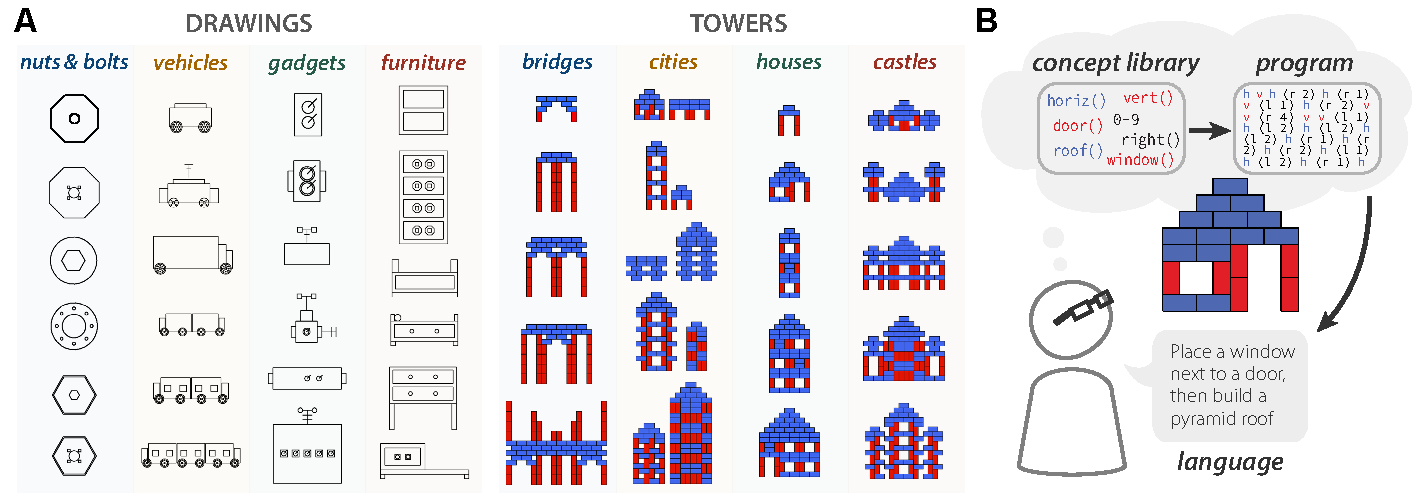
\includegraphics[width=0.99\linewidth]{figures/lax_task.pdf}
  \caption{(A) Example objects from the technical-drawing and block-tower domain. Each domain contains 4 subdomains consisting of 250 examples each. Each domain and subdomain was designed to include high variation over the type and number of base primitives (i.e., shapes, blocks). (B) This work aims to infer the latent concept library that people are using to decompose complex objects into parts, where objects are represented by executable graphics programs.}
  \label{fig:task}
  \end{center}
 \end{figure*}



% In this paper,  we suggest that the \textit{level of abstraction} people choose when describing a domain of compositional objects -- like the \textit{technical drawings} and \textit{block towers} in Fig. \ref{fig:task}A -- can be modeled as a \textit{DSL choice} over possible libraries of formal conceptual primitives at differing levels of abstraction, which can be composed into generative programs to produce any chosen object. We hypothesize that the level of abstraction reflects a contextual tradeoff between \textbf{DSL size} (the total number of concepts necessary to represent objects in a given domain, using a particular set of conceptual primitives) and \textbf{program description length} (how many primitives in the chosen DSL must be composed to describe any individual item drawn from the domain). This hypothesis formalizes an intuitive tradeoff in classical, part-based theories of the basic level: a low-level set of parts (like describing the drawing in terms of \textit{squares} and \textit{circles}) uses a small vocabulary, but requires  many words to describe an individual object; a high-level but specific set of parts (one with specialized terms for different makes and models of dressers, for instance) might succinctly describe any one object, but at the expense of requiring a large overall vocabulary to describe a diverse domain.

% To evaluate this, we develop a dataset of two domains of hierarchical object stimuli (Fig. \ref{fig:task}A), and conduct a procedural language experiment to elicit human descriptions of each object. We find that people use different, context-specific linguistic vocabularies dependent on the subdomain of objects (Part I). We then introduce the formal representational approach, defining program \textit{DSLs} at varying levels of abstraction, that we use to model abstraction choice in language. Using this, we first use \textit{program description length} alone to correlate programs and language (Part II), and discuss findings and challenges of this approach. Finally, we introduce a more expressive \textit{program-language alignment} model, and find that people's language is best explained in this model by DSLs that jointly minimize program description length \textit{and} overall DSL size (Part III).



\section{Part I: Eliciting procedural descriptions \\ of object structure} \label{sec-part-i}
% Consider how you might describe the drawing or block tower in Figure \ref{fig:task}A. Both images could be described in language that carves up the image, intuitively, at multiple levels of abstraction -- how would you choose between describing the drawing using a simple but low-level vocabulary of basic strokes (like \textit{lines, circles, and squares}) vs. a set of names for some of its functional parts (like \textit{antenna} or \textit{dial}); or between describing the block tower as composed of \textit{red blocks} and \textit{blue blocks} vs. of higher-level parts like a \textit{roof} and \textit{floors}?

% All we know about this dataset is that it has STRUCTURE; what we expose is variation in nameability. 

% Extend from holistic judgements and labeling to more detailed descriptions of object structure.
% lots of parts
% lots of structure

% We begin by developing a large dataset of two domains of hierarchical object stimuli (Fig. \ref{fig:task}A) and a procedural language experiment to elicit human descriptions of each object.
% In this section we investigate the basic claim that people are able to flexibly describe object structure, and establish a correspondence between linguistic descriptions and conceptual representations.
% While the overarching aim of this paper was to investigate how people talk about the compositional structure of objects, we also wanted to explore how context affects the concepts we use to represent and talk about objects-- particularly the level of abstraction our concepts occupy.
% We therefore needed a set of stimuli that a) had varied compositional structure, b) could be divided into multiple distinct categories (i.e. contexts), and c) was constructed from a set of simple elements that could be combined at various levels of abstraction.

% How do people describe the compositional structure of complex objects across varied domains?
% And how does context affect the level of abstraction that people use to represent objects?
% To study these questions, 

A core motivation for this work is to propose and validate a general approach to identifying the library of part concepts that people invoke to decompose objects. 
Towards this end, we needed a large and varied enough collection of objects, and a naturalistic task for eliciting detailed descriptions of their structure. 
In Part I, we describe our strategy for synthesizing a diverse collection of novel objects and encouraging human participants to thoroughly describe the parts they contain. 
We also report insights from our analysis of how well a ``base'' graphics library containing only the simplest shape primitives could explain how many words and which words people used.

% To gain traction on the question of how people robustly communicate about object structure, we first developed a large and varied collection of structured object stimuli and elicited natural-language descriptions of them. % (Fig.~\ref{fig:task}A).
% In this section, we describe our stimulus  and task procedure, and evaluate a basic correspondence between the language participants used to describe our stimuli and the program representations that underlie their construction.

\subsection{Methods}

\paragraph{Participants}
465 participants recruited from Prolific completed the task. 
Participants provided informed consent and were paid approximately \$15 per hour. % for their time.

% (A) Example linguistic descriptions for objects from each domain. (B)
% \textbf{TODO: Add back examples as panel A on the left, but with substantial compression. Re-format text by concatenating what/where content.} 
\begin{figure*}[ht!]
  \begin{center}
  \includegraphics[width=0.99\linewidth]{figures/lax_description_length_and_word_distribution.pdf}
  \caption{(A) Relationship between length of base-library programs and length of linguistic descriptions. (B) \textit{Left:} Top-10 words that appeared most frequently in descriptions for each domain. \textit{Right:} Top-10 words with highest pointwise mutual information (PMI) within each subdomain.}
  \label{fig:words}
  \end{center}
\end{figure*}

\paragraph{Stimuli} 

% To accomplish this, we constructed two domains of stimuli-- (\textit{technical drawings} and \textit{block towers}) (Fig. \ref{fig:task}A)-- that are each generated from a shared base set of procedural, symbolic primitives (shapes or blocks).
% We then ran an experiment to elicit language from subjects who were familiarized with stimuli from a specific \textit{subdomain}-- each containing items generated from distinct generating procedures over these primitives and varying hierarchically in terms of their compositional parts.
% We hypothesized that the vocabularies people used to describe each stimulus would be \textit{context-specific}: that participants would tend to use different vocabularies tailored to the subdomain distribution of stimuli they were shown.

% different motivation for artificial stimuli: XXX
% Don't need to talk about nameability: say it has structure
% We expose variability in structure (x-axis in part II)
% While many such categories exist in the real world, these often come with canonical ways of being decomposed into parts, or have a hierarchical structure that is too ambiguous to permit the formal modeling approach of \ref{sec-part-ii}.

% To construct a set of stimuli with variation in compositional structure, 

% todo: tie to program abstraction
% Desiderata: 1) varied set of categories, 2) hierarchical structure; 3) primitives + higher-order abstractions available to describe, 4) novel + evocative
% 	What do these buy us?
% #1 more general findings
% #2 reminiscent of hierarchical structure of real-world concepts
% #3 allows us to test the notion of "basic-level" but for parts (Rosch et al.) (“just right” level of abstraction)
% #4 lets us look at learning (later)
% why drawings? why block towers?

To ensure that we had a large enough collection of objects that varied in the kind and amount of structure they contain, we developed a hierarchical procedure for synthesizing complex configurations of shapes. 
Taking inspiration from recent work employing line drawings and block towers to investigate how people learn and represent the the compositional structure of objects \shortcite{tian2020learning, mccarthy2021learning,wang2021learning}, we defined two stimulus \textit{domains}, distinguished by the set of base shape primitives used to generate them (Fig.~\ref{fig:task}A).
\textit{Drawings} were composed of simple geometric curves (i.e., line, circle) and evocative of familiar object categories; \textit{Towers} were composed of rectangular blocks (i.e., horizontal and vertical dominoes) and evocative of simple architectural models.

To investigate the degree to which people invoked category-specific part concepts to describe these objects, rather than the same set of ``atomic'' base primitives in all cases, we further defined four \textit{subdomains} nested within each domain. 
Within \textit{Drawings}, we informally designated these as \textit{nuts \& bolts}, \textit{vehicles}, \textit{gadgets}, and \textit{furniture}; and within \textit{Towers}, \textit{bridges}, \textit{cities}, \textit{houses}, and \textit{houses} (Fig.~\ref{fig:task}A).
For each subdomain, we procedurally generated 250 unique examples, hierarchically composing the base primitives into increasingly complex, recursively defined parts. 
A \texttt{dresser}, for example, was composed of \texttt{drawers}, which are in turn composed of a \texttt{panel} and \texttt{knobs}, and which are themselves defined by combining \texttt{circles} and \texttt{lines}.
In sum, this procedure yielded a collection of 2000 novel objects that spanned a wide range in visual complexity: 1000 Drawings and 1000 Towers, each accompanied by a graphics program that could be used to regenerate it in terms of the base primitives.

% Alongside each stimulus, generative models also emitted a corresponding \textit{program}, expressed in a domain-specific language, that fully specified a procedure for recreating the stimulus from the set of base primitives shared across its \textit{domain}.
% We enumerated stimuli for each subdomain, and selected a random but biased sample of each to obtain 250 stimuli of varying complexity for each subdomain.

% two domains were further divided into four \textit{subdomains}, each defined by a distinct generative model that was hand-designed to produce objects of a recognizable subordinate category (e.g., \textit{furniture}, \textit{castle}) from a set of predefined abstractions (e.g., \textit{legs}, \textit{towers}).

% Our stimulus set was divided into two distinct \textit{domains}, each procedurally generated from a different set of base primitives (Fig.~\ref{fig:task}A):
% \textit{technical drawings} were designed to resemble schematic drawings of functional objects and were composed of simple geometric shapes; 
% \textit{block towers} were designed to resemble simple architectural models and were composed of 2D rectangular blocks.
% Each of the two domains were further divided into four \textit{subdomains}, each defined by a distinct generative model that was hand-designed to produce objects of a recognizable subordinate category (e.g., \textit{furniture}, \textit{castle}) from a set of predefined abstractions (e.g., \textit{legs}, \textit{towers}).

% Generative models consisted of a set of nested, parametric functions operating over the base primitives, hierarchically composing them into increasingly complex, recursively-defined parts.
% A \textit{dresser}, for example, is composed of \textit{drawers}, which are in turn composed of a \textit{panel} and \textit{knobs}, and which are defined finally over a shared set of simple shape primitives.
% Alongside each stimulus, generative models also emitted a corresponding \textit{program}, expressed in a domain-specific language, that fully specified a procedure for recreating the stimulus from the set of base primitives shared across its \textit{domain}.
% We enumerated stimuli for each subdomain, and selected a random but biased sample of each to obtain 250 stimuli of varying complexity for each subdomain.

\paragraph{Task procedure}

Each participant was instructed to provide step-by-step instructions for how to ``draw'' or ``build'' 10 different objects sampled from a \textit{single} subdomain, such that someone else could reconstruct each one based on their description.
% Each participant produced descriptions for 10 items drawn from a single \textit{subdomain} (e.g., only \textit{castles}). 
% To gain familiarity with the task-relevant distribution of stimuli and part abstractions, participants first clicked through 25 images of other stimuli from the same subdomain.
At the beginning of each session, participants were first familiarized with the general characteristics of the that subdomain by viewing 25 examples (none of which then appeared during the main experiment).
Throughout the session, they were also shown the upcoming 7 objects they would be asked to describe, to provide them with concurrent information about how objects varied within the subdomain.
% However participants were not encouraged to produce instructions that disambiguated their items from others in their domain, as in a traditional reference game.
Because we are primarily focused on interrogating which part descriptors people invoke, we designed the text-entry interface to encourage participants to describe each step by composing a \textit{what}-phrase and a \textit{where}-phrase, which were entered into separate text boxes. 
Participants could include as many instruction steps as they deemed necessary and there was no time limit on each trial.

% which  language referring to parts distinct from language referring to spatial relations. 
% \textit{what} they would draw/place \textit{where}
% designed the text-entry interface with two separate : a \textit{where} 
% the language used to refer to the parts of an object from spatial descriptions of where those parts should go, participants typed each step of their procedure into a pair of \textit{what} and \textit{where} text boxes, describing what should be drawn/placed where, in order, to reproduce the target image. 

\paragraph{Language preprocessing} % spacy, en_core_web_lg,
To investigate the content of the instructions generated by participants, we use the spaCy NLP library to extract and lemmatize words, using part-of-speech (POS) tagging to remove determiners and punctuation. We also replaced common typos (``sqaure,'' ``cirlce,'' etc.) and spelling variations (``centre,'' ``colour,'' etc.) with their canonical spellings in US English.

\subsection{Results}
% ($b=XXX$, $t=XXX$, $p=XXX$)
% $XXX\%$ (95\% CI: $[XXX, XXX]$)

\paragraph{People use more words to describe more complex objects (up to a point)}
% We first set out to establish whether participants' language was sensitive to the distribution of objects they were describing.
% The high degree of variation in stimulus complexity provided a natural opportunity to explore the relationship between the relationship between the number of simple shape elements in an object and how many words participants used to describe it. 
%%%%%%% 
% We ran a linear mixed effects models with fixed effects for domain and trial number, an interaction term between the two, as well as random intercepts for subdomain and participant.
% \textit{Block tower} instructions were longer than those for \textit{technical drawings}, both in terms of the number of \textit{what-where} steps  ($b=5.08$, $t=10.9$, $p<0.001$) and raw character counts ($b=373$, $t=8.24$, $p<0.001$). 
% We suspected that this was due to participants identifying a greater number of distinct entities in the \textit{block tower} stimuli, which was supported by a greater number of words entered in the \textit{what} boxes of \textit{block towers} than for \textit{technical drawings} ($b=25.8$, $t=9.55$, $p<0.001$).
% Together, these results confirm that participants' descriptions were sensitive to the kinds of items they were describing, but what about the stimuli themselves explains this variation in language? 
%%%%%%%
The high degree of shape variation in our stimulus set provided us with a natural opportunity to explore the relationship between the complexity of an object and the length of the linguistic description participants provided for it.
Insofar as participants display a tendency to decompose objects into a consistent number of parts, regardless of how complex these parts are, the length of their descriptions would be predicted to remain stable over a wide range in object complexity. 
Alternatively, if participants tend to decompose objects into a set of commonly recurring parts, and provide instructions for each one, the length of their descriptions would be predicted to positively correlate with object complexity. 
A third possibility is that there is a systematic but non-linear relationship between object complexity and linguistic description length \cite{sun2021seeing}, consistent with a compromise between the first two strategies. 
% has suggested a systematic but non-linear relationship between this measure of  object complexity and the length of their linguistic descriptions \cite{sun2021seeing}.
% , which was consistent with initial observations in our data (Fig. \ref{fig:words}A).
% To test this hypothesis more rigorously, we operationalized natural-language description length using the mean number of words entered in the \textit{what} text boxes and operationalized the program length as the number of tokens required to express that object in the base DSL.
% To test this hypothesis more rigorously, we fit a mixed-effects model to predict the length of each natural-language description, including fixed effects of the object's subdomain (with eight levels) and the corresponding program length in the base DSL.

For these analyses, we operationalize object complexity as the length of the graphics program that generated it using the base primitives and measure the length of linguistic descriptions as the number of words provided in the \textit{what} text boxes only.
To tease apart the above possibilities, we fit a mixed-effects model to predict linguistic description length from graphics program length (Fig. \ref{fig:words}A), including random intercepts for participants and random effects of program length at the participant level.
% and effects of program length at the participant-level. %the number of program tokens required to recreate the object (Fig. \ref{fig:words}A).
We observed a significant main effect of program length, $t(318)=14.8, p < 0.001$ across all subdomains (Fig.~\ref{fig:words}B), providing evidence against the possibility that participants invoke part concepts of arbitrary complexity in order to provide instructions of the same length. 
We also found that a model including an additional quadratic effect of program length, allowing for a non-linear relationship, significantly improved the fit, $\chi^2(3)=38.6$, although the strength of this relationship varied across subdomains.
These findings suggest that people generally use more words to describe more complex objects, but the strength and nature of this relationship can vary widely across object categories. 
Moreover, even the best-fitting quadratic model failed to capture a large proportion of the variation in language using only program length as a measure. % written only in terms of simple shape primitives.

% Nevertheless, it appeared that instructions produced for both domains spanned a range of levels of abstraction (Fig. \ref{fig:words} A), with some referring to lower level primitives (i.e. geometric shapes and individual blocks) and some to more abstract compositions of these lower elements (e.g. ``desks'', ``pillars'', and ``castle-like block towers'').
% Stimuli from each domain were constructed from distinct sets of base primitives that can be combined according to distinct sets of constraints, allowing us to investigate whether participants systematically varied their vocabulary according to their context.

% n_steps ~ domain * trial_num + (1 | subdomain) + (1 | gameID)
%                              Estimate Std. Error         df t value Pr(>|t|)    
% (Intercept)                   4.36409    0.33821    8.47840  12.904 7.25e-07 ***
% domainstructures              5.07991    0.46552    7.58715  10.912 6.61e-06 ***
% trial_num                    -0.06105    0.02143 4183.00156  -2.848  0.00442 ** 
% domainstructures:trial_num   -0.29242    0.02878 4183.00156 -10.162  < 2e-16 ***


% char_sum ~ domain * trial_num + (1 | subdomain) + (1 | gameID)
% Fixed effects:
%                           Estimate Std. Error       df t value Pr(>|t|)    
% (Intercept)                 305.566     32.635    7.475   9.363 2.16e-05 ***
% domainstructures            373.091     45.288    6.922   8.238 8.04e-05 ***
% trial_num                    -5.493      1.640 4182.994  -3.350 0.000817 ***
% domainstructures:trial_num  -29.624      2.201 4182.994 -13.457  < 2e-16 ***


% n_whats_filtered ~ domain * trial_num + (1 | subdomain) + (1 |      gameID)
%                             Estimate Std. Error        df t value Pr(>|t|)    
% (Intercept)                  17.6224     1.9618    7.9137   8.983 2.01e-05 ***
% domainstructures             25.8495     2.7060    7.1447   9.553 2.53e-05 ***
% trial_num                    -0.2667     0.1174 4182.9953  -2.272   0.0231 *  
% domainstructures:trial_num   -1.5601     0.1576 4182.9953  -9.900  < 2e-16 ***


\paragraph{People use different words to describe different objects} % Looking at content rather than length

While none of the items in our stimulus set look exactly like real-world objects and buildings, several of them are nevertheless \textit{evocative} of familiar visual categories (e.g., vehicles, furniture, houses). 
Insofar as these associations guided their language behavior to some extent, participants may have used different words to describe the parts of objects from different subdomains. 
Alternatively, if people referred exclusively to low-level shape primitives common to all subdomains within a given domain, then we would not expect there to be large differences in the kind and relative frequency of words people produced. 
To tease apart these possibilities, we aggregated tokens produced by all participants for objects in each subdomain and computed the pointwise mutual information (PMI) for each word, providing a measure of the strength of association between a given word and subdomain (Fig.~\ref{fig:words}B).
% which provides a measure of the strength of the association between a given word and  
% (as opposed to the full domain; we consider the domains independently.) 
% We aggregate the preprocessed instructions across each subdomain and compute the pointwise mutual information (PMI) of each word with respect to each subdomain (as opposed to the full domain; we consider the domains independently.) 
% These PMI values were estimated using a Laplace smoothing metric to eliminate extremely low-frequency words (n $\leq$ 5). %; full analysis code is released at the code repository.
This analysis revealed several words that were used often within a particular subdomain, but not in others (e.g., \textit{drawer}, \textit{leg}, and \textit{knob} in the \textit{furniture} subdomain), suggestive that certain part concepts may be specific to subdomain. 
%%% JSD analysis
To quantitatively evaluate whether there was a difference in participants' word choice across subdomains, we computed the Jensen-Shannon distance (JSD) between the word frequency distributions aggregated across all trials in each subdomain, and compared this value to a null distribution of random assignments of trials to subdomain groups.
We found that mean distance between subdomains was significantly greater than between random assignments to subdomains (\textit{Drawings}: $d = 0.439$, $p < 0.001$; \textit{Towers}: $d = 0.328$, $p < 0.001$), supporting the hypothesis that participants relied on different words to describe the parts of objects from different subdomains.
The larger JSD value for Drawings further suggests that the subdomains of Drawings elicited more distinct descriptions compared to those of Towers. %any interpretation needed here?
% DOMAIN-LEVEL JSD: To estimate how dissimilar language was across domains, we computed the Jensen-Shannon distance (JSD) between the word frequency distributions aggregated across all trials in each domain, and compared this value to a null distribution of random assignments of trials to domains.
% We found that the distance between word distributions at the domain-level was significantly greater than would be expected by chance ($d = 0.736$, $p<  0.001$).
% Similarly, when we instead aggregated over subdomains, we found that mean distance between subdomains was significantly greater than between random assignments to subdomains (\textit{Drawings}: $d = 0.439$, $p < 0.001$; \textit{Towers}: $d = 0.328$, $p < 0.001$).
Taken together, these exploratory analyses indicate that people used a wide variety of terms, in many cases using words that correspond to the parts of real-world objects, rather than to simple graphics primitives.
Moreover, we discovered that people often used different words to describe otherwise visually similar objects, although this was more pronounced for the \textit{Drawings}.


% This is further supported by computing the F-statistic to measure within-cluster variance, comparing word-count vectors labeled with a given subdomain to randomly-assigned subdomain labels. 

% However, examining the relative word frequency distribution produced greater discriminability by subdomain for \textit{technical drawings} ($\Delta F = 12.5$, 95\% CI: [$9.46$, $16.0$], $p<0.001$) than for {block towers} ($\Delta F = 1.47$, 95\% CI: [$0.0441$, $2.83$], $p=0.088$). 

% We find that the \textit{technical drawing} subdomain labels explain cluster variance signficantly better than random assignments ($\Delta F = 12.5$, 95\% CI: [$9.46$, $16.0$], $p=0$); this effect is not significant for subdomain labels in the \textit{block towers} domain ($\Delta F = 1.47$, 95\% CI: [$0.0441$, $2.83$], $p=0.088$).

% We conduct a preliminary linguistic analysis of subdomain-level vocabulary variation. 

% Fig. \ref{fig:vocabulary_gallery}A (left, black) shows the top 10 words ordered by their \textit{base counts} across each whole domain, contrasted by the top-10 words ordered by \textit{PMI} for each subdomain (right columns, colored), indicating the usage of words (eg. \textit{drawer}, \textit{leg}, and \textit{knob} in the \textit{furniture} subdomain) suggestive of subdomain-specific part structure. 

% Fig. \ref{fig:library_gallery}B also shows TSNE-visualizations of word-count vectors constructed for each stimulus, suggesting that there may be greater subdomain-level language differentation in the \textit{technical drawings} domain than in the \textit{block towers} domain. This is further supported by computing the F-statistic to measure within-cluster variance, comparing word-count vectors labeled with a given subdomain to randomly-assigned subdomain labels. We find that the \textit{technical drawing} subdomain labels explain cluster variance signficantly better than random assignments ($\Delta F = 12.5$, 95\% CI: [$9.46$, $16.0$], $p=0$); this effect is not significant for subdomain labels in the \textit{block towers} domain ($\Delta F = 1.47$, 95\% CI: [$0.0441$, $2.83$], $p=0.088$).


\section{Part II: Aligning procedural descriptions and conceptual abstractions}\label{sec-part-ii}
The variation in words used across subdomains suggests that people represent and often prefer to use subdomain-specific \textit{part concepts} to describe our stimuli. Tasked with describing a large set of related objects drawn from a highly-structured subdomain, they readily pick out and name part concepts like \textit{knobs} and \textit{drawers}, or 
\textit{windows} and \textit{doors}. How do they choose this particular lexicon: what determines \textit{how many}, and \textit{which} part concepts, they name?

In this section, we now formalize this problem as a search over the space of \textit{possible graphics libraries} that can be used to represent each subdomain. We introduce a \textit{library abstraction} procedure used to construct a hypothesis space of alternative \textit{graphics libraries} containing parts at varying levels of complexity, based on the parametric structure of each subdomain's original generative model. We then use introduce a \textit{library-to-vocabulary alignment} metric using a model from the statistical machine translation literature, which measures how well programs written in each library predict the language people actually use for each subdomain.

Together, these modeling approaches allow us to formalize a hypothesis about part representation in language: that people name part concepts corresponding to graphics libraries tailored to each subdomain, which provide both efficient compression of the objects they are describing while \textit{also} minimizing the size of the graphics library itself.

% The variation in vocabularies used across subdomains suggests that participants represented objects in our dataset using higher-level of abstractions than the library of base primitives used to define them. N

%% SEARCH OVER LIBRARIES
% In this section, we turn from instance-level descriptions to subdomains: how do speakers choose a \textit{lexicon} of words and part concepts to describe the subdomain as a whole?

% Building on our modeling approach from Part I -- which correlates individual stimulus instructions and stimulus programs using a \textit{description length} metric -- we introduce two analogous modeling techniques: a \textit{DSL abstraction} procedure, which allows us to construct higher-order DSLs based on subdomain part structure; and a \textit{DSL-vocabulary alignment model}, used to measure correspondences between entire vocabularies and program DSLs.

% We use this extended model to formalize a hypothesis that links linguistic vocabularies to latent \textit{subdomain-level} structure: we expect that speakers tailor their vocabularies across the subdomain to reflect both the representational cost of \textit{individual stimuli} (based on individual program description lengths) and of the \textit{subdomain as a whole} (based on the size of the DSL containing all program concepts across the subdomain.)

\subsection{Methods}
\paragraph{Constructing a space of abstract graphics libraries}
%% This will probbably be subsumed in the introduction.
The generative models for each subdomain described in Part I are highly structured. However, the corresponding \textit{programs} they emit are written from the same \textit{base library} of simple, low-level primitives (\textit{blocks} and \textit{shapes}) across each subdomain. These programs are also verbose: they must compose a large number of base primitives to represent the higher-order \textit{part concepts} (such as \textit{knobs} and \textit{wheels}, or \textit{pillars} and \textit{roofs}), that humans seem to name.

We can, however, extract \textit{higher-order libraries} that abstract out the nested, parametric functions used to generate each subdomain. Formally, these higher-order DSLs rewrite the program for each stimulus in terms of concise program abstractions: chunked subroutines representing repeated part structure (such as \textit{wheel} or \textit{roof} components) shared across a given subdomain
(see Fig. \ref{fig:library_gallery}). Each of these libraries represents a \textit{hypothesis} about a possible part decomposition for the subdomain: by constructing several such libraries, we can ask which best predicts the words people actually use.


Our top-down DSL extraction procedure is analogous to the automated, bottom-up \textit{program library learning} methods in \shortcite{ellis2020dreamcoder, tian2020learning, mccarthy2021learning}, which discover subroutines from a dataset of programs that often correspond qualitatively to domain-relevant concepts.
% However, with access to each subdomain's hierarchical generation procedure, we can construct these DSLs directly.
However, in this work, we chose to construct DSLs manually, allowing us to consider a wide range of abstraction levels while maintaining a high degree of fidelity to the procedures by which the stimuli were originally generated.

We extract three higher-order DSLs ($L_1$, $L_2$, $L_3$, visualized in Fig.~\ref{fig:library_gallery}) that coarsely bucketize subdomain structure into three levels of increasing abstraction. By construction, components in successively higher-order DSLs build recursively on those at the previous level: for instance, the components in $L_1$ contain chunked subroutines that abstract directly over the base DSL (\textit{lines} to \textit{polygons}); and components in $L_2$ abstract additionally over those in $L_1$ (\textit{polygons} to \textit{rows of polygons}). 


\begin{figure}[t]
  \begin{center}
  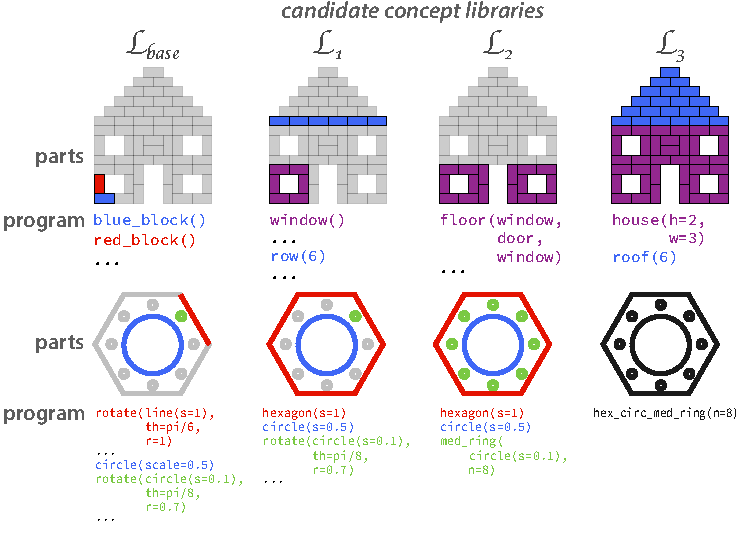
\includegraphics[width=0.99\linewidth]{figures/lax_libraries.pdf}
  \caption{Each DSL contains additional abstractions...}
  \label{fig:library_gallery}
  \end{center}
\end{figure}

\paragraph{Library-to-vocabulary alignment model}
The DSLs constructed in the previous section specify a hypothesis space of alternative \textit{subdomain-level} representations at differing levels of abstraction. We can now ask: which (if any) of these DSLs best describes the linguistic vocabulary speakers use for each subdomain? 

% We formalize this notion of lexical correspondence with a \textit{vocabulary-DSL alignment metric} that leverages token-token statistical alignment models used to relate parallel language datasets in machine translation. Here, we use these models to derive an aggregate metric of how closely program components in a given DSL co-occur with words across each subdomain.

We formalize this notion of lexical correspondence with a \textit{vocabulary-DSL alignment metric} that reflects how closely program components in a given DSL co-occur with words across each subdomain. To compute this metric, we leverage IBM Model 1 \shortcite{gal2013systematic}, a standard machine translation model which can be fit to paired programs and instructions to estimate token-token translation probabilities $P(w_i|\pi_j)$ (for each word $w_i$ in the linguistic vocabulary and program component $\pi_j$ in a DSL). For each subdomain, we evaluate each DSL $L_i$ using a cross-validation scheme (with batches of n=5 held out stimuli). We fit the model to all but the held out stimuli and evaluate the \textit{mean per-word log-likelihood} for each held out instruction given its stimulus program in DSL $L_i$. We use \textit{mean token log-likelihood} (which correlates monotonically with negative {perplexity} \shortcite{wu2016google}) to normalize for instruction lengths. For comparison with Part I, we consider only the pre-processed `what' instructions for each stimulus.

% \begin{figure*}[!ht]
%   \begin{center}
%   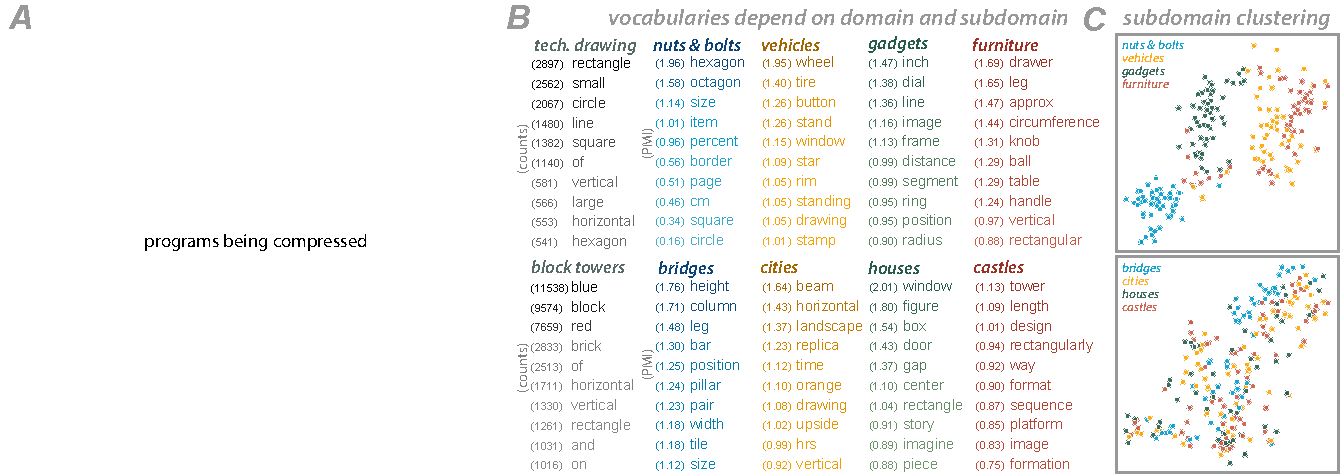
\includegraphics[width=1.0\linewidth]{figures/lax_vocabularies.pdf}
%   \caption{(A) Word counts for domain. PMI for subdomains. (B) Clustering of word-count vectors shows more distinct language across subdomains of technical drawings than of block towers. Each point is a participant, each of whom described items in a single subdomain. (C) }
%   \label{fig:vocabulary_gallery}
%   \end{center}
% \end{figure*}


\begin{figure*}[ht!]
  \begin{center}
  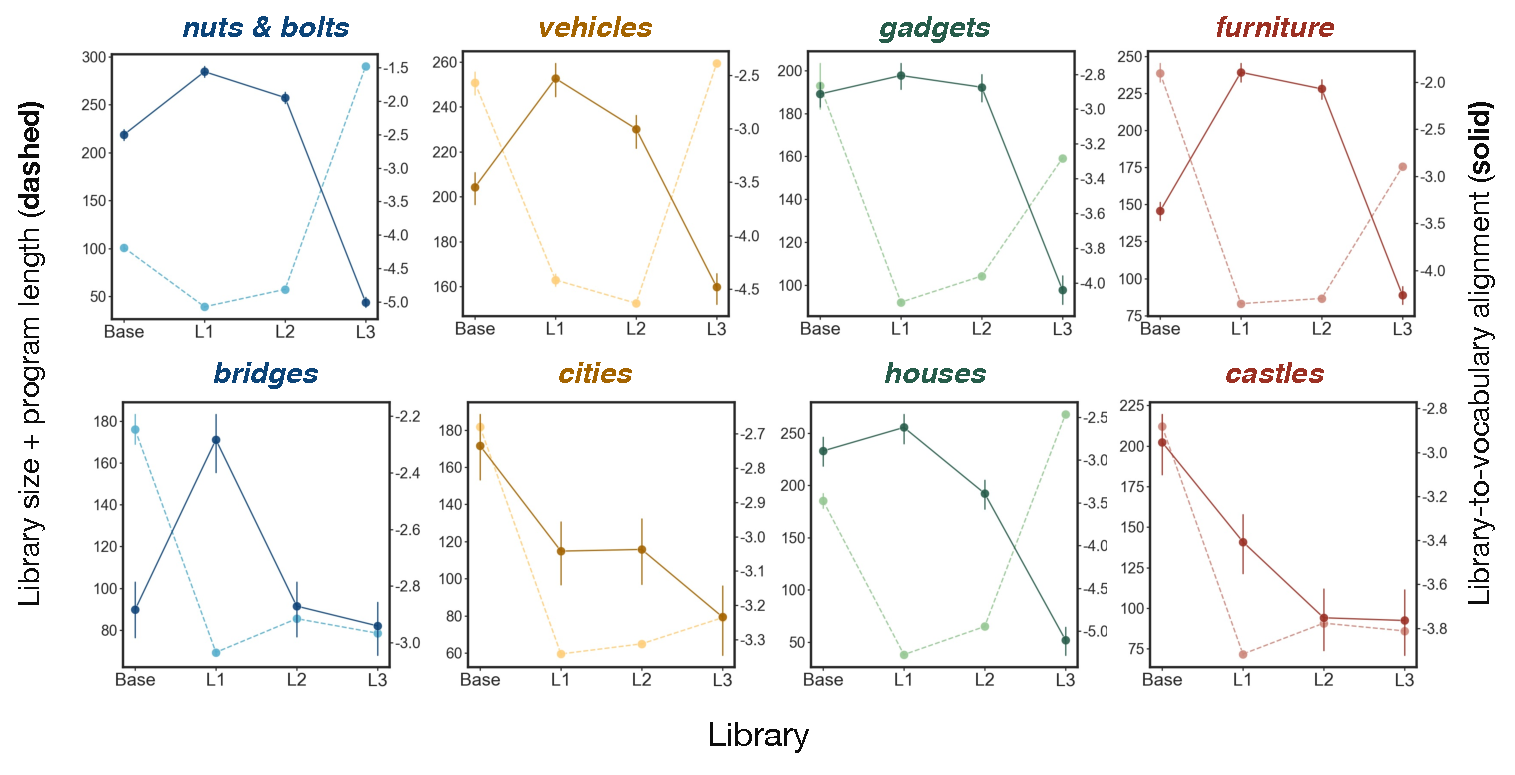
\includegraphics[width=0.9\linewidth]{figures/lax_library_costs.pdf}
  \caption{[SCRATCH] 
  Perplexity (blue, left y-axis) and combined DSL size and program length (red, right y-axis) within each subdomain; shown with respect to DSL size; DSL size increases with additional higher-level abstractions. Shown for the base DSL, $L_1$, $L_2$, and $L_3$.}\label{fig:perplexity-length}
  \end{center}
\end{figure*}

\subsection{Results}
\paragraph{Moderately complex libraries best compress objects while minimizing library size} 
Our DSL extraction procedure reflects a subdomain-level tradeoff in representational cost: higher-order DSLs \textit{compress} programs for individual stimuli (Fig. \ref{fig:library_gallery}B), as each program can be written using a smaller number of subdomain-specific part abstractions. However, each higher-order DSL is subsequently larger than the last: it adds more unique, subdomain-specific abstractions.
% (and following earlier work, such as \shortcite{mccarthy2021learning, ellis2020dreamcoder}, we add new abstract components cumulatively while retaining their lower-level components in the DSL). 
This tradeoff between program description length $|\pi|$ and library size $|L|$ is well-described in prior DSL-learning models \shortcite{ellis2020dreamcoder}, and is closely analogous to the information-theoretic, optimal compression problems described in \shortcite{kirby2015compression} -- referring to increasingly subdomain-specific components trades off concision in describing any one stimulus with the total number of concepts necessary to describe the whole domain. 

As DSL-size $L$ grows monotonically with level of abstraction ($L_{\text{base}} \leq L_1 \leq L_2 \leq L_3$), Fig. \ref{fig:perplexity-length} (dashed line) plots this combined representational cost $C_L = |L| + \sum_{\pi \in \mathcal{D}}{|\pi|}$. This reveals a characteristic non-monotonic trend: $C_L$ is minimized in intermediate-level DSLs and increases in the base DSL (when programs are long) and in the highest-order DSLs (when the number of subomdain-specific abstractions overwhelms gains in program compression).

\paragraph{Peoples oderately complex libraries}
We can finally consider the formal \textit{DSL-vocabulary alignment} metric in relation to our original, subdomain-level hypothesis. Fig. \ref{fig:perplexity-length} (solid line) plots the \textit{mean-log-likelihoods} under the DSL-vocabulary alignment model (higher indicates words are better predicted by DSL components) for each subdomain, along the same $L$ x-axis.

We first confirm that this metric identifies certain DSLs which align significantly better to the vocabulary than others. A one-way ANOVA finds that there is a strongly significant difference (p $<$ 0.001) in mean-log-likelihoods between DSLs, in all subdomains. 

In all but two of the subdomains (\textit{cities} and \textit{castles}), Fig \ref{fig:perplexity-length} (dashed) shows that our DSL-vocabulary metric not only varies non-monotonically over the higher-order DSLs, but is maximized for intermediate DSLs. Comparing optima between mean log-likelihood (solid) and the combined DSL and program length (dashed) supports our overall hypothesis: DSLs that better explain language (increasing mean log-likelihood in the program-language alignment model) correspond closely with those that minimize, or approximately minimize, the joint representational cost $|$L + program length$|$.


\subsection{Discussion}

%%%% SUMMARY %%%%
Language provides a window onto the way we extract and represent structure in the world.
In this paper, we elicit linguistic descriptions for a large dataset of richly structured stimuli, and present a formal approach to linking descriptions with object structure through the programs used to generate them.
We find that the length of people's descriptions of objects varied with the lengths of their generative programs, establishing a basic correspondence between language and object structure.
We also find that the content of these descriptions was sensitive to the higher-order compositional structure of the objects, allowing us to investigate more structured relationships between the words people use and higher-order conceptual abstractions, operationalized as program abstraction.
In particular, we find evidence that language is generally better explained by programs that include higher-order abstractions, but that concept libraries are sensitive to a trade-off between the amount of abstractions to be remembered and the cost of representing objects with that library.

%%%% WIDER CONTRIBUTION %%%%

(Wider contribution: XXX)


%%%% FUTURE DIRECTIONS 1: FOLLOW-UP ON INTERPRETABILITY  %%%%


Linguistic abstraction can provide a way of capturing more information in fewer words, however this process can also be lossy.
In future work, we aim to measure how robustly linguistic descriptions describe the stimuli by presenting them to naive participants and measuring performance on a series of reconstruction tasks.
% asking them to pair parts of the descriptions with parts of the objects.
% reconstruct the stimuli from the set of base primitives.

% more data/ ppts?

%%%% FUTURE DIRECTIONS 2: CONTEXT %%%%

The idea that people favor a \textit{basic level} of abstraction -- one adaptively selected as a "just right" level of abstraction dependent on context -- is well-documented in both word choice and non-linguistic object identification tasks \shortcite{brown1958shall, rosch1976basic}.
%communicative goal
One such form of contextual variation is the speaker's communicative goal.
The requirement of communicating an interpretable procedure, kept constant in this study, may favor fine-grained procedural representations, compared to contexts in which communicating about an object's identity is more important.
Reference games are a well-studied example of such a context, and would provide a salient alternative to compare to the results presented here.

% individual learning
%   =>  Pre-post study: individual non-linguistic experience vs. individual language usage
One empirical observation not reported above was evidence of a decrease in description length over time. 
A possible explanation for this phenomenon, suggested by prior work involving a collaborative block-tower assembly task \cite{mccarthy2021learning}, is a linguistic shift towards higher level of abstraction over time.
How people acquire new procedural abstractions, and the extent to which language use modulates such learning, is an avenue for future work.


% How contextual is the level of abstraction? 
%   => Collect more data for item-specific and speaker-specific variation
%   => Modulate size of domain even more

% How does shared experience modulate the level of abstraction?
%   => Paired tasks (CA++)


%%%% ZOOMED OUT %%%%
(zoomed out: XXX )


% \paragraph{Model-based DSL identification meaningfully distinguishes between DSLs that better explain language.} We first verify that our method meaningfully differentiates between DSLs of differing sizes. Stat: Reject null hypothesis of flat line. ANOVA: compare means between all DSLs.

% \paragraph{Learned abstractions generally explain language better than the base DSL, and intermediate DSLs explain language better than the most abstract DSLs.}
% (What about the two cases where it does not? Room for error.) Except for the two domains where DSLs do not improve on perplexity, Fig. 1A shows that the DSL which yields the best perplexity is L1, and that perplexity falls off after, formalizing a ‘basic level’. Why is it L1? Room to shift the prior. 

% STATS: Nested model confirms that there is a non-linear trend (how to report this?) - quadratic fits better than linear.

% \paragraph{DSLs that better explain language minimize base DSL size and program length.} Finally, Fig [BOTTOM ROW] shows |Base DSL| + |program length|.
% STAT: Is there some way to say this other than pointing at the graphs?


% \paragraph{People adapt the abstractions they use contextually to the subdomain.} We hypothesized that higher-level DSLs, containing context-specific abstractions, would always better predict language in each subdomain. Our results in Fig.  \ref{fig:language_libraries}A suggest that this is generally true, along with a more nuanced interpretation: in \textit{most} of the subdomains, a contextual DSL improves perplexity under the translation model as compared to the base DSL. However, in two of the block towers subdomains --  the \textit{cities} and \textit{castles} domain, in fact the base DSL yields the best perplexity. 

% This result suggests that people do indeed adapt the level of abstraction they use in language, dependent contextually on the subdomain of stimuli -- after all, while the base DSL can be used to describe \textit{every} subdomain (eg. people could \textit{always} have described each structure in terms of its low-level blocks), people seem to have chosen it selectively for some domains and other, more context-specific abstractions for others.

% What explains when people fall back on the base DSL of primitives? A visual inspection of the \textit{cities} and \textit{castles} abstractions suggests one intuitive explanation: the availability of commonly-understood linguistic terms to describe these abstractions. While our results in many domains suggest that people flexibly pick out higher-level, contextual abstractions -- and adapt their vocabulary to reflect them -- humans performing a naive procedural description task, intended for other naive speakers, are also constrained by the basic English terms available to them. We see these results as especially promising for ad-hoc \textit{convention formation} paradigms [CITE], to determine whether subjects can \textit{further} adapt their language to a context with additional joint experience.

% \paragraph{People generally choose an intermediate level of abstraction.} Our secondary hypothesis suggests a tradeoff between contextual-abstraction -- which reduces the cost of describing any given stimulus in a subdomain -- and vocabulary size, modeled by the size of each enriched DSL. Our results in Fig.  \ref{fig:language_libraries}A support this conclusion, finding a characteristic U-shaped curve for the domains where more abstract DSLs better predict language: perplexity in the translation model does not increase monotonically with abstraction level (and DSL size.)

% However, as with the previous finding, this result suggests a promising avenue for future work to disentangle the cause of this trend: does this curve reflect an individual choice on the part of the speaker (to take into account the cost of a larger vocabulary), or a limit in the contextual abstraction afforded by language intended for naive listeners (which permits some variation in abstraction level, but may not contain sufficiently interpretable terms as abstrations grow more context specific)? Again, we see this as an especially promising route for considering language between paired speakers in an extended joint conversational context.


% People choose flexibly between different levels of abstraction and specificity in language -- we might switch between referring to our \textit{car} to distinguish it from other modes of transportation, and referring to our \textit{orange minivan} to pick it out from other models at a parking lot.


\bibliographystyle{apacite}

\setlength{\bibleftmargin}{.125in}
\setlength{\bibindent}{-\bibleftmargin}

\bibliography{CogSci_Template}


\end{document}
